\chapter{Úvod do problematiky Laser Game systému}

\section{Laser Game}
Laser Game, někdy také nazývána i Laser Tag, je označení pro společenské hry, motivované sci-fi, využívající moderní elektroniku. Hráči získávají body za zásahy infra červeným paprskem z jejich zbraně do zásahových čidel soupeřů či jiných objektů vybavených zásahovým čidlem. A naopak o své body přicházejí, jestliže se jejich zásahová čidla stanou terčem nepřátelských IR paprsků. Cílem každého hráče je získat co nejvíce bodů.

Nejčastěji se hra odehrává v místnosti speciálně upravené pro tento účel, označované jako aréna. Stěny, strop a podlaha arény bývají zpravidla pokryty tmavou barvou (černé koberce, koženky a podobné materiály) tak, aby se zabránilo odrazům IR paprsků. Zdi v arénách jsou často vypolstrovány, aby se snížilo riziko zranění hráčů. Obvykle arény nejsou jen klasické místnosti se čtyřmi stěnami a rovnou podlahou, nýbrž často bývají značně členité, vybavené úkryty a překážkami.

Pro zpestření hry mohou být arény vybaveny i další elektronikou, například optickými závorami, minami či světelnými nebo kouřovými efekty.

\section{Historie Laser Game}
Koncem sedmdesátých a na začátku osmdesátých let vyvíjela firma Lockheed Martin Information Systems pro armádu Spojených států amerických systém, využívající IR paprsky pro trénink boje, nazývaný \zkratka{MILIES}. Systém funguje na stejném principu jako \zkratka{LG}. Voják má na hlavni zbraně IR vysílač, který reaguje na stisk spouště. Voják je oděn ve speciálním obleku s IR senzory. Při zásahu vojáka jsou odeslány z obleku informace do řídící jednotky, která vyhodnotí, zda je voják zraněn či virtuálně mrtev - používání tohoto systému je bezpečnější než využití konvenčních zbraní. V roce 1992 vyšla nová verze tohoto systému pojmenovaná MILIES2000, která navíc po virtuální smrti vojáka zablokuje jeho další střelbu a akusticky ohlásí zasažení. \zkratka{MILIES} využívá od roku 2002 i Armáda České republiky a také i ostatní země s \zkratka{NATO}.

Prvním komerčně prodávaným zařízením, se kterým je spojován vznik \zkratka{LG}, je hračka Star Trek Electronic Phaser od společnosti South end Electronics, která byla uvedena na trh v roce 1979. Hračka má tvar futuristické zbraně inspirované Star Trekem. Součástí zbraně je signalizační blok, který pomocí LED a reproduktoru indikuje zásah. A blok střelby vybavený IR vysílací LED.

\section{Laser Game systém}
\zkratka{LG} systém je soustava zahrnující \zkratka{HW}, \zkratka{FW} a \zkratka{SW} umožnující hrát \zkratka{LG}. Tento systém lze tedy chápat jako vybavení nezbytné pro provozování celé arény.

Nejdůležitějšími součástmi \zkratka{LG} systému jsou vesty, zbraně, komunikační směrovač a řídící \zkratka{PC}, \zkratka{LG} systém může být dále doplněn například o optické závory, miny či bomby.

\begin{figure}[H]
    \begin{center}
        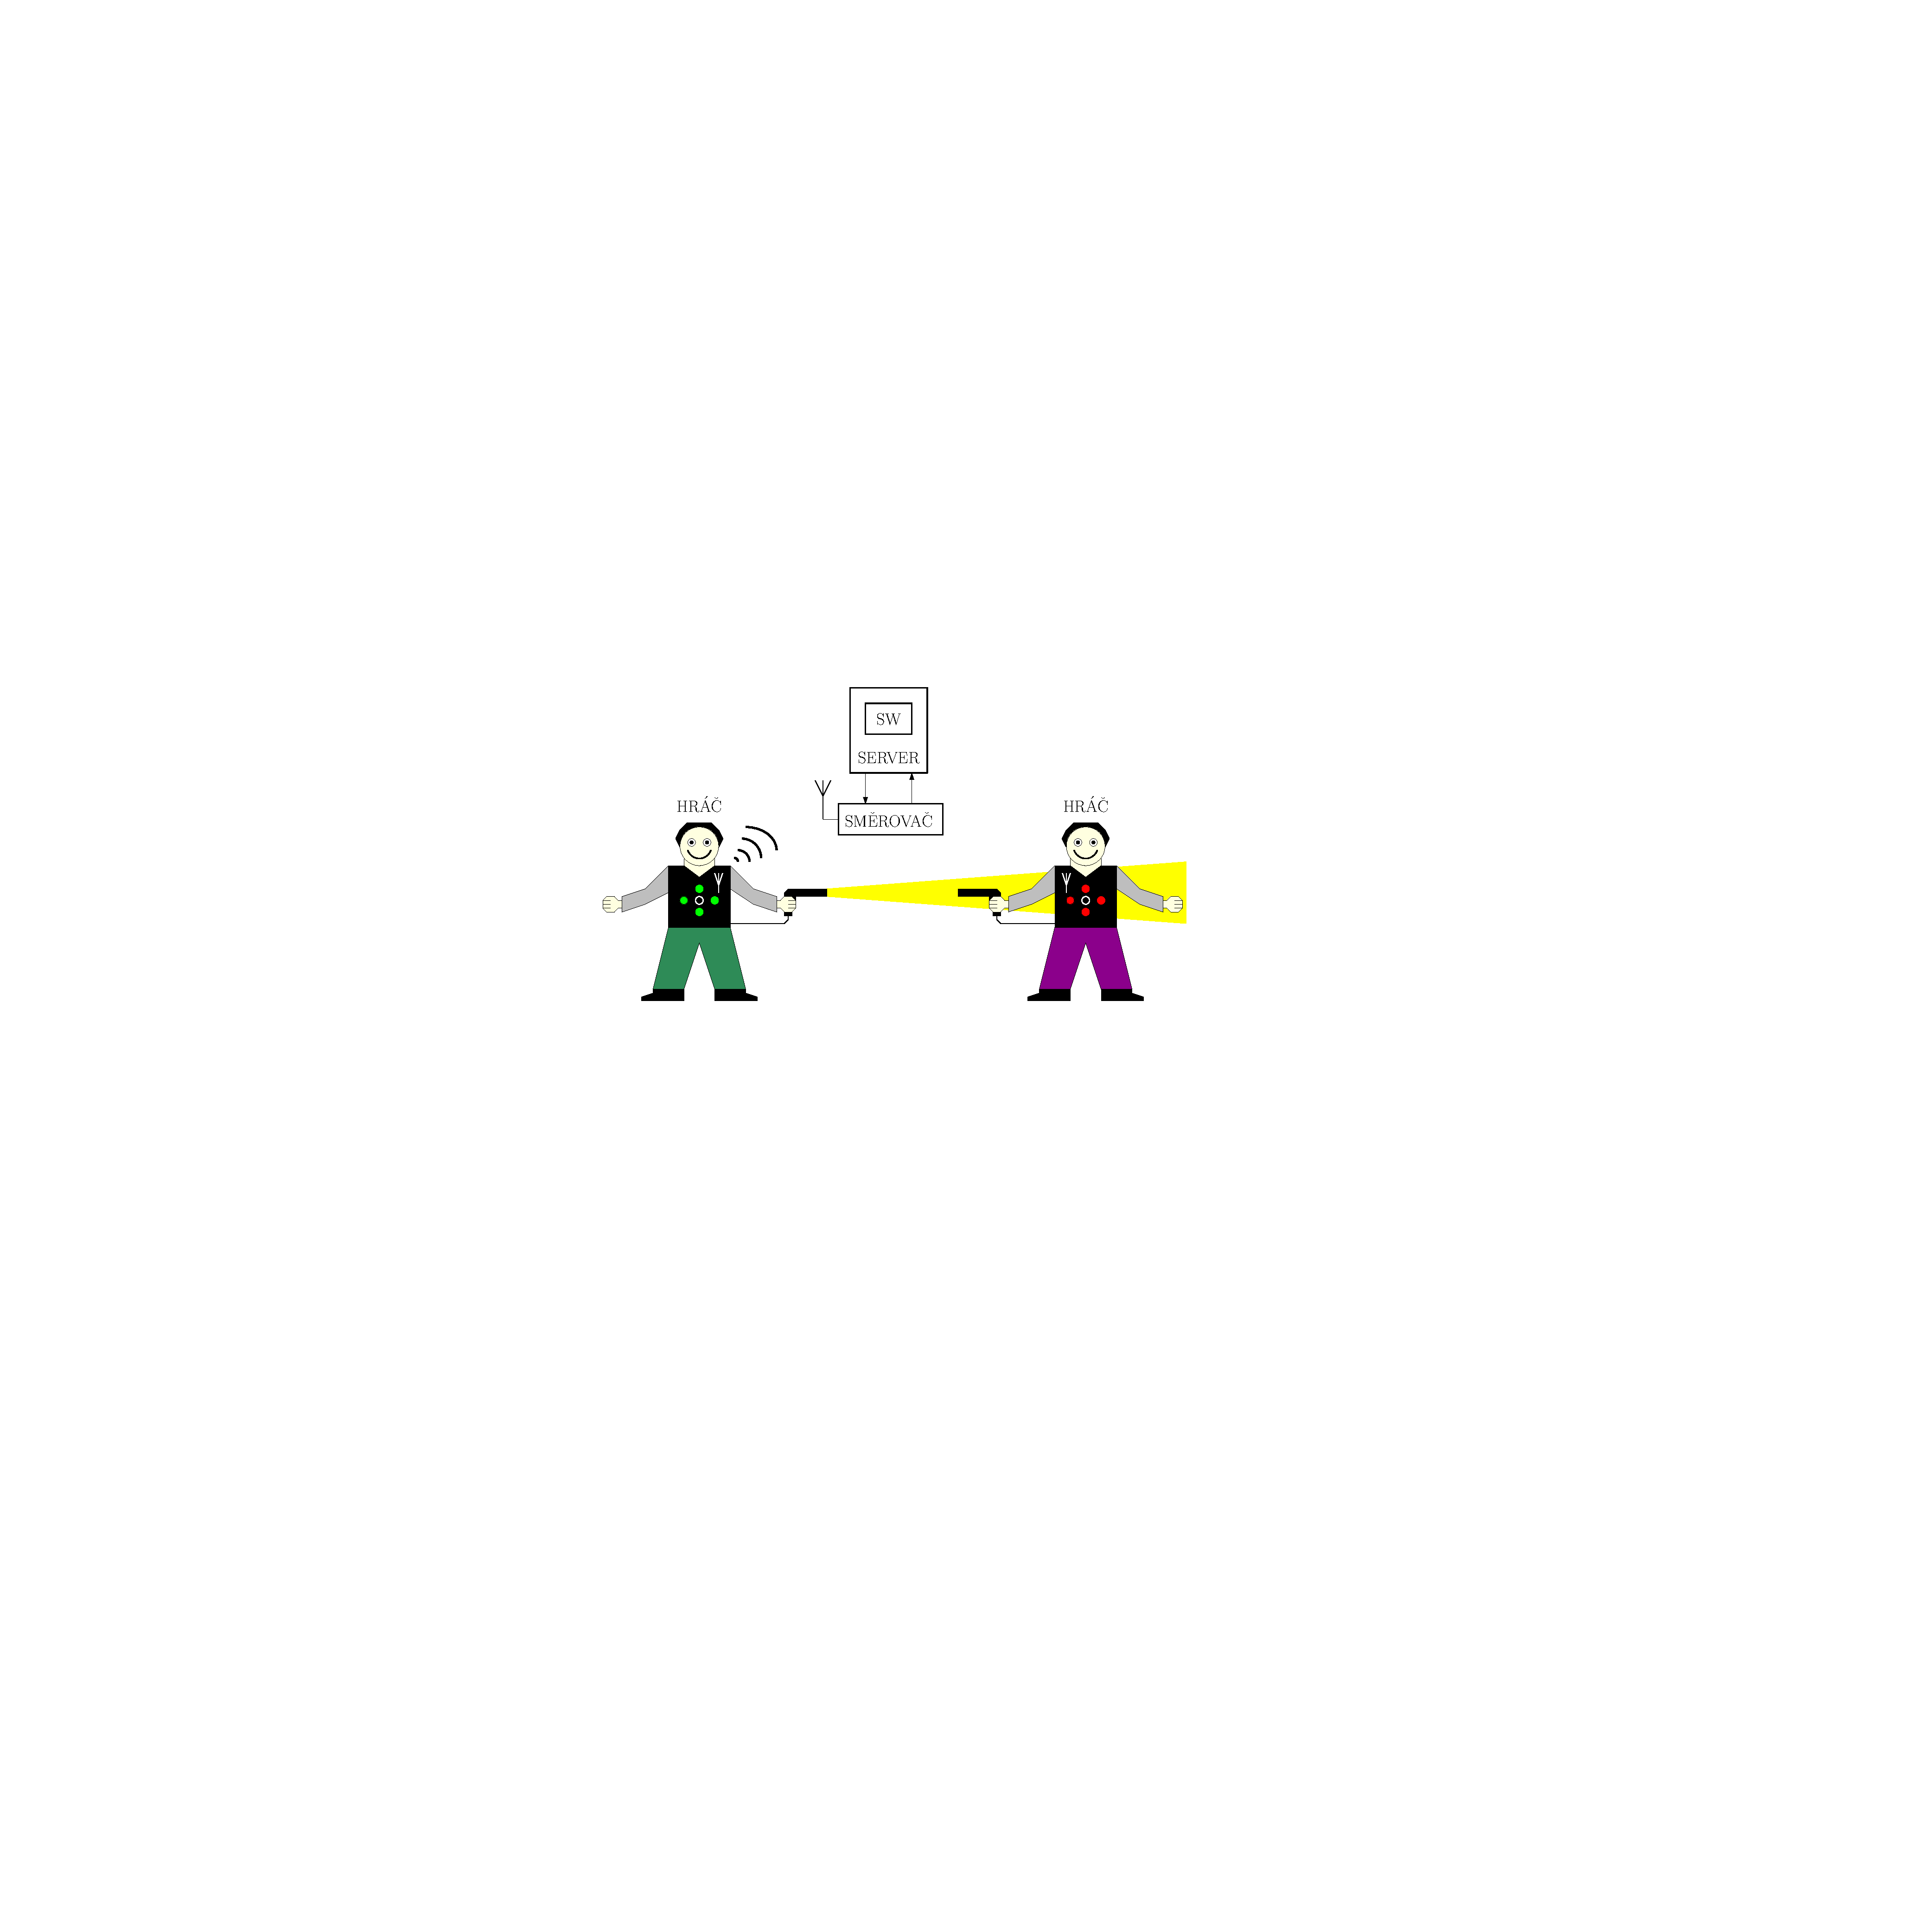
\includegraphics[width=\textwidth]{img/lgs}
    \end{center}
    \caption{Znázornění \zkratka{LG} systému}
\end{figure}

\paragraph{Řídící počítač}
má za úkol prostřednictvím směrovače komunikovat s vestami, případně i dalšími zařízeními v síti. Hostuje řídící \zkratka{SW}, pomocí něhož operátor arény ovládá hru. Zajišťuje nakonfigurování vest, v průběhu hry stahuje z vest aktuální údaje a vyhodnocuje pořadí hráčů. Často bývá doplněn tiskárnou, díky níž po vyhodnocení hry vytiskne statistiky z právě odehrané hry.

\paragraph{Směrovač}
zajišťuje směrování v bezdrátové síti - zprostředkovává tedy duplexní spojení mezi vestami a počítačem.

\paragraph{Vesta}
je oděv, který nosí hráči - má dvě hlavní funkce, detekovat zásahy a komunikovat s řídícím počítačem. Další funkcí vesty je barevná identifikace hráčů pomocí RGB LED. Vesta může zajišťovat i zvukové efekty, či zobrazovat hráči jeho statistiky z aktuální hry. Vesta také komunikuje se zbraní hráče a vyhodnocuje, jestli může daný hráč střílet. Existují řešení, kdy je vesta nahrazena systémem tagů upevněných na oblečení, tato varianta ale není moc oblíbená vzhledem k tomu, že upevňování tagů je zdlouhavé a během hry hrozí jejich odpadnutí.

\paragraph{Zbraň}
má jednoduchou úlohu, zajišťuje vysílání IR paprsku, který při zásahu vesty způsobí virtuální zabití hráče. Také může obsahovat IR detektor, díky kterému může být signalizováno poškození zbraně jejím zásahem. Dále může být i zbraň vybavena signalizační RGB LED pro identifikaci týmu, svítilnou či displejem.
